\section{High Productivity with ISI}
The goal of ISI is to allow the simultaneous \emph{simulation},
\emph{prototyping} and \emph{validation} of a system during development.
Figure~\ref{easy} illustrates the ISI method on a high level. Like the
four-step development method described in the previous section, ISI includes
simulation, prototyping and measurement, but design, implementation and
validation are implicit by-products. In section~\ref{sec:case-study}, we shall see an example on
how this can be achieved. An essential requirement of ISI is that the real world
is modeled \emph{as is}. This, of course, is usually not possible, but domain
specific abstractions apply as in all models. This requirement stems from the
fact that in order for the components of the simulation to be usable as
prototypes, they should implement \emph{real-world} logic as much as possible.

\begin{figure}[htb]
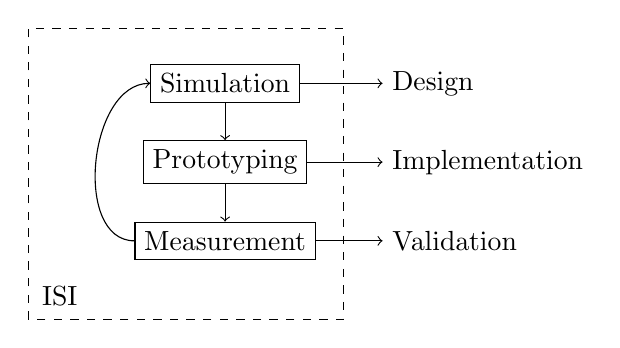
\begin{tikzpicture}
	\node[draw] (Simulation) at (0,2) {Simulation};
	\node[draw] (Prototyping) at (0,1) {Prototyping};
	\node[draw] (Measurement) at (0,0) {Measurement};

	\node (ISI) at (-2.1,-.7) {ISI};
	\draw[dashed] (-2.5,-1) -- (-2.5,2.7) -- (1.5,2.7) -- (1.5,-1) -- (-2.5,-1);

	\node[anchor=west] (Design) at (2,2) {Design};
	\node[anchor=west] (Implementation) at (2,1) {Implementation};
	\node[anchor=west] (Validation) at (2,0) {Validation};

	\draw[->,draw] (Measurement) to[in=180,out=180] (Simulation);
	\draw[->,draw] (Simulation) to (Design);
	\draw[->,draw] (Prototyping) to (Implementation);
	\draw[->,draw] (Measurement) to (Validation);

	\draw[->,draw] (Simulation) to (Prototyping);
	\draw[->,draw] (Prototyping) to (Measurement);
\end{tikzpicture}
\caption{A high-level description of the ISI architecture}
\label{easy}
\end{figure}

\subsection{Process-based Modeling}
For ISI to be applicable the model must be decomposed into distinct and
independently communicating parties or \emph{processes}. As the world is highly
concurrent, decomposition is rarely an issue, but the inverse is. Limiting
concurrency is an issue that PDES approaches must deal with, customarily done
by mapping multiple \emph{physical} processes to one \emph{logical} process.
This has the disadvantage of coupling the previously distinct processes. This can
often be optimized, but still represents an engineering challenge.

In the context of a storage system, a natural decomposition into distinct
processes is ``simply'' to identify the concurrent interactions that take
place, i.e. the issuing of I/O requests from clients, handling by a cache, the
latency introduced by switches etc.

For ISI to be effective, an environment that allows millions of concurrent
processes is required. This can be achieved through direct language support
(such as present in Erlang\cite{erlang}, Go\cite{Go} or
occam-$\pi$\cite{occam-pi}) or through libraries such as ZeroMQ\cite{zeromq} for
languages lacking direct support. Here, we employ Go, which is Google's
emerging concurrent programming language. Go is in part influenced from C,
occam, Limbo\cite{limbo} and Newsqueak\cite{newsqueak} and includes
language-level concurrency primitives such as light-weight processes called
\emph{goroutines}, first-class communication channels and the
\verb|select|-statement which allows non-deterministic choice
(pseudo-random) from a set of possible send or receive operations. Go is
designed to be highly productive and easy to learn. It does so, by promoting
convention over convenience and using a relatively small number of syntactic
elements compared to e.g. C++. Go is generally not considered to be an
object-oriented language, and uses another approach compared to other
languages. Methods are allowed on \emph{any} type and does not use the notion
of a \emph{class}. To implement dynamic dispatch, Go provides \emph{interface}
types that are compatible with any type implementing the methods described in
the interface\cite{goref}.

While the concurrency features of Go were influenced from CSP and the $\pi$-calculus,
it cannot be uniquely categorized. The concurrency features are often discussed
in the context of CSP, but Go's channels are more akin to the $\pi$-calculus
because channels may be communicated over channels. On the other hand, Go does not
allow guards in \verb|select|-statements.

To an observer the different processes are completely sequential and blocking
in nature. The process receives a message, handles it and (optionally)
replies with an answer. We find that this programming model is simpler to
understand than what is known as the \emph{callback hell}\cite{callback-hell} arising from
asynchronous single-threaded event handling, known from building concurrent
services in languages that don't provide light-weight process support (e.g.
JavaScript).

\subsection{Tracking Time}
\label{sec:tracking-time}
As described in section~\ref{sec:diff-comp}, ISI does not impose any specific
method for tracking time, but for ISI to be applicable to a broad range of
systems, we need to discuss how to handle causality. We are not interested in
ever handling reverse events as is needed in the previously mentioned Timewarp
PDES algorithm.  Doing so would eliminate the point of ISI; that simulation and
implementation is interchangeable. A prototype should not have to handle a
causality violation. It won't happen in real life.

Instead, some concepts from conservative PDES are elegant solutions for
communicating processes. Given a process $p$, that handles
requests for connected peers $a_i$, one approach is to ensure that all $a_i$
always has at least one message queued at $p$. These messages can be actual
requests, or if the process is simulating a period of inactivity, a
message indicating the how long. This ensures that $p$
can handle requests for all remaining processes, without violating causality,
but does require a process' peers to be static. The technique is not as
straight-forward as it sounds and does require special \emph{null}-messages
(with no other purpose than updating a clock) to avoid deadlocks. The
conservative PDES approach in general, as well as why \emph{null}-messages are
required to avoid deadlocks, are beyond the scope of this paper, but see Misra's
1986 paper\cite{dist-des} for a thorough description and proof of correctness.

While the conservative approach is universal and could be built into an ISI
library, we will argue in section~\ref{sec:case-study}, that not all
simulations or systems require these extra messages, justifying our choice that
ISI should not handle causality implicitly.

\subsection{Simulation as Measurement}
A distinctive feature of ISI is that real-time measurement is done at the same
points as where simulation happens. The only change needed to transition from
simulation to measurement is to swap the randomized timings common in event
simulations with an actual timing around an actual operation. This
substantially decreases the time from simulating a system to testing a
prototype in the lab because the prototype is implicitly designed and
implemented through the development of the simulator.

The implicit support for measurement in the prototype also makes testing and
verifying the system model uncomplicated and ensures that the final system is
capable of doing statistics at reference points which, through simulation, was
found to be important for reasoning about the system.

Similarly, as described in section~\ref{sec:tracking-time}, periods of
inactivity are handled in simulation by sending messages about inactivity to
peers. An action that is simply disabled when moving to measurement, because
this is now handled by actual waiting for resources or replies.

\subsection{Validation}
In our storage simulator, a workload generator produces a stream of synthetic
I/O requests. As the simulator evolves, so does a system capable of handling
these I/O requests in a real setting. To validate and reason about the
precision of the simulation, simulated actions of components can be gradually
swapped for real actions. The result of processing request in real-time
provides valuable feedback to our software such that simulated durations can
be tuned.  This is the iterative process that was described in the introduction.

Thus, validation can be regarded as part of the development work flow, but it
does not require a separate validation engine; the built-in measurements are
sufficient.
